\section{Power Dissipation}

%\makelabheader %(Space for student name, etc., defined in master.tex)

\bigskip

\textbf{Extra Apparatus}
\begin{itemize}[nosep]
\item digital multimeters (2)
\item DC power supply 
\item various resistors
\item banana cables and alligator clips
\end{itemize}

\bigskip

\begin{enumerate}[wide]

\item Your DMM has three different ranges for DC current measurement, and two different input jacks to plug in the leads for these measurements.  How do you know which input jack and which ranges to use?  What happens if you get it wrong?

\item Get several extra resistors (of different sizes) from the front of the room.  All of these should have a resistance of about 100 $\Omega$.  Measure their resistances precisely.  For each resistor, make a table in your lab notebook like the one below.   Now hook each one up to the big DC power supply with alligator clips (NOT using your breadboards), and slowly increase the voltage of the power supply.  At each voltage setting, measure the current through the resistor and the voltage across the resistor precisely, using two separate DMMs.  Your actual voltage values will be slightly different from 1.0, 3.0, etc.  From your measurements, calculate the actual resistance, and the power dissipated in the resistor at each setting.  Also feel the resistor carefully to see if it is getting hot.  When you are done with each resistor, let it cool and measure its resistance one last time with the DMM.  Was there any permanent change?  
\begin{enumerate}
\item What is the difference between the physically large and physically small resistors?
\item How do your observations compare with the nominal power rating for each resistor?
\item Is the temperature coefficient of each of these resistors positive or negative?  (That is, does the resistance increase or decrease as a function of temperature?)
\end{enumerate}

\begin{center}
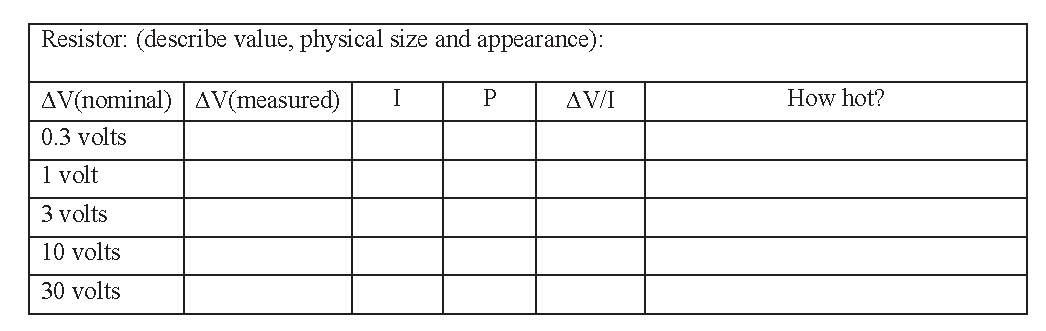
\includegraphics[width=1.0\textwidth]{power/iv_table.eps}
\end{center}

Be sure to check in with the instructor after completing the table for your first resistor, to catch any misunderstandings before doing all of them!
\end{enumerate}


\textbf{Possible Exam Questions:}

\begin{itemize}
\item Describe a specific set of current and voltage measurements you could make of a resistor to determine whether it had a positive or negative coefficient.  Give an example of numbers for a set of current and voltage measurements that would be consistent with a negative temperature coefficient.
\end{itemize}





